\subsection{Slučaj upotrebe: Pregled rezultata}

\subsubsection*{Kratak opis}
Student pregleda objavljene rezultate završenih izbora ili, ukoliko izbori nisu uspeli, obaveštenje o ponavljanju izbora.

\subsubsection*{Akteri}
\begin{itemize}
    \item \textbf{Student} -- pregleda rezultate izbora.
\end{itemize}

\subsubsection*{Preduslovi}
\begin{itemize}
    \item Student je prijavljen u sistem.
    \item Period glasanja za izabrane izbore je završen.
\end{itemize}

\subsubsection*{Postuslovi}
\begin{itemize}
    \item Student je upoznat sa ishodom izbora.
    \item Stanje sistema se ne menja.
\end{itemize}

\subsubsection*{Osnovni tok}
\begin{enumerate}
    \item Student bira završene izbore i opciju \textbf{Rezultati}.
    \item Sistem proverava status izbora.
    \item Ako je izborna komisija objavila rezultate, sistem prikazuje procenat izlaznosti i broj glasova koji je dobila svaka izborna lista.
    \item Student pregleda rezultate.
\end{enumerate}

\subsubsection*{Alternativni tokovi}
\begin{enumerate}[label=\textbf{A\arabic*.}]
    \item \textbf{Izbori se ponavljaju.} Ako je u koraku 2 izborna komisija objavila obaveštenje o ponavljanju izbora, sistem prikazuje obaveštenje da izbori nisu važeći zbog nedovoljne izlaznosti i da će biti ponovljeni.
    \item \textbf{Rezultati još nisu objavljeni.} Ako u koraku 2 izborna komisija još nije objavila ni rezultate ni obaveštenje, sistem prikazuje poruku da rezultati još nisu objavljeni.
\end{enumerate}

\begin{figure}[H]
    \centering
    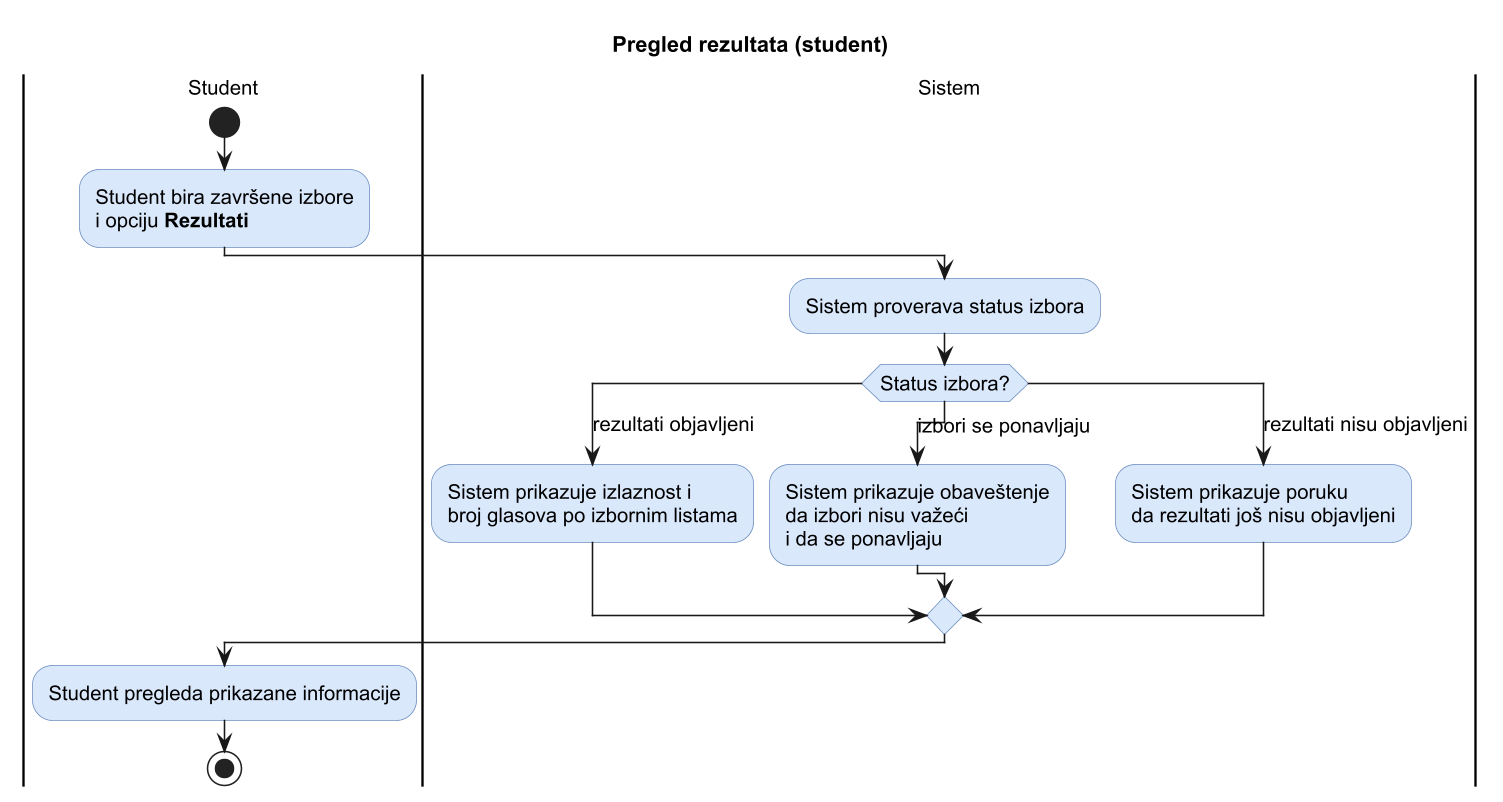
\includegraphics[width=\textwidth]{aktivnosti_pregled_rezultata.png}
    \caption{Dijagram aktivnosti: Pregled rezultata}
    \label{fig:pregled_rezultata}
\end{figure}

\newpage
